
\documentclass[14pt,aspectratio=169,usenames,dvipsnames]{beamer}

%%%%%%%%%%%%%%%%%%%%%%%%%%%%%%%%%%%%%%%%%%%%%%%%%%%%%%%%%%%%%%%%%%%%%%%%%%%%%%%%

    \usepackage[english]{babel}
    \usepackage[utf8]{inputenc}
    \usepackage[T1]{fontenc}
    \usepackage{lmodern}
    \usepackage{textcomp}
    \usepackage[cm]{sfmath}
    \usepackage[euler]{textgreek}
    \usepackage{xfrac}
    \usepackage{tikz}
    \mathchardef\mhyphen="2D

    %% Set the left and right margins
    \usepackage{changepage}
    \setbeamersize{text margin left=4.5em,text margin right=2.5em}

    %% Fonts
    \setbeamerfont{title}{series=\bfseries,size=\huge}
    \setbeamerfont{subtitle}{series=\bfseries,size=\large}
    \setbeamerfont{date}{size=\footnotesize}
    \setbeamerfont{frametitle}{series=\bfseries,size=\large}
    \setbeamerfont{block title}{series=\bfseries,size=\large}
    \setbeamerfont{footline}{size=\normalsize}

    %% Colors
    \usebackgroundtemplate{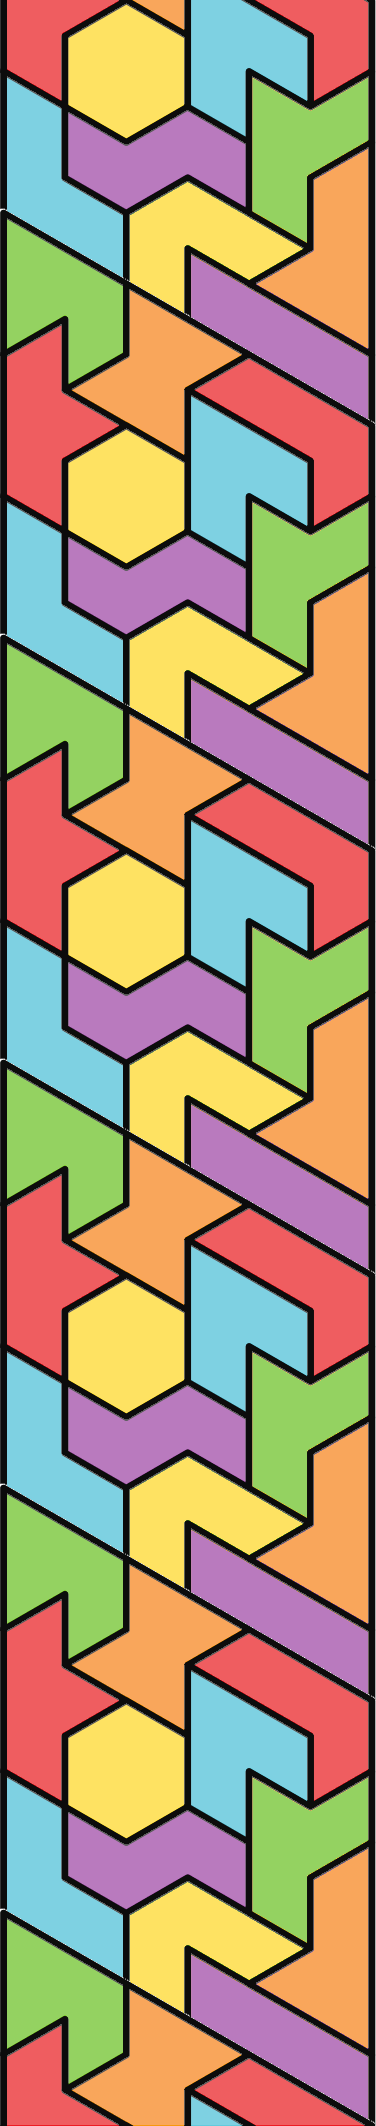
\includegraphics[height=\paperheight]{pictures/Barra Hex.png}}
    \setbeamercolor{background canvas}{bg=white}            % Blackboard
    %\setbeamercolor{structure}{fg=NavyBlue}
    \setbeamercolor{structure}{fg=black}
    \usebeamercolor{structure}
    \setbeamercolor{normal text}{fg=structure.fg}

    %% Add a line after the frametitle
    \setbeamertemplate{frametitle}[default][left,leftskip=2.15em]
    \addtobeamertemplate{frametitle}{}{\vspace*{-1ex}\rule{1.\textwidth}{2pt}}

    %% Use circular discs as itemized list markers
    \setbeamertemplate{itemize items}[circle]

    %% Remove default navigation symbols
    \setbeamertemplate{navigation symbols}{}

    %% Remove the footline
    \setbeamertemplate{footline}{}

    % MMACa Logo
    \setlength{\fboxsep}{3pt}
    \setlength{\fboxrule}{0.75pt}


%%%%%%%%%%%%%%%%%%%%%%%%%%%%%%%%%%%%%%%%%%%%%%%%%%%%%%%%%%%%%%%%%%%%%%%%%%%%%%%%

\title{\LARGE{El diseño del Tangram Egipcio}\vspace{-0.5em}}
\author{
    \includegraphics[height=18ex]{figures/figure001a.pdf}\\[-0.25ex]
    {\small \href{https://creativecommons.org/licenses/by-nc-sa/4.0/}{
\includegraphics[scale=0.15]{pictures/cc.pdf}
\includegraphics[scale=0.15]{pictures/by.pdf}
\includegraphics[scale=0.15]{pictures/nc.pdf}
\includegraphics[scale=0.15]{pictures/sa.pdf}} \href{https://github.com/CarlosLunaMota}{Carlos Luna-Mota}}\\
    \vspace{0.55em}
    \href{https://mmaca.cat/}{
\includegraphics[height=3ex]{pictures/logo.png}}
    %\href{https://mmaca.cat/}{\large \framebox{\textbf{mmaca}}}\\
    \vspace{-1.85em}}
\date{}

\begin{document}

    %%%%%%%%%%%%%%%%%%%%%%%%%%%%%%%%%%%%%%%%%%%%%%%%%%%%%%%%%%%%%%%%%%%%%%%%%%%%

    \begin{frame}
        \titlepage
    \end{frame}

    %%%%%%%%%%%%%%%%%%%%%%%%%%%%%%%%%%%%%%%%%%%%%%%%%%%%%%%%%%%%%%%%%%%%%%%%%%%%

    \begin{frame}{}
        \begin{center}
            \textbf{\huge El Tangram...}
        \end{center}
    \end{frame}

    %%%%%%%%%%%%%%%%%%%%%%%%%%%%%%%%%%%%%%%%%%%%%%%%%%%%%%%%%%%%%%%%%%%%%%%%%%%%

    \begin{frame}{Tangram - Dinastia Song (960-1279)}
        \begin{center}
            \includegraphics[height=20ex]{figures/ffigura001.pdf} \\
        \end{center}
    \end{frame}

    %%%%%%%%%%%%%%%%%%%%%%%%%%%%%%%%%%%%%%%%%%%%%%%%%%%%%%%%%%%%%%%%%%%%%%%%%%%%

    \begin{frame}{Tangram - Siluetas}
        \begin{center}
            \includegraphics[height=15ex]{figures/ffigura002a.pdf} \quad \includegraphics[height=15ex]{figures/ffigura002b.pdf} \\
        \end{center}
    \end{frame}

    %%%%%%%%%%%%%%%%%%%%%%%%%%%%%%%%%%%%%%%%%%%%%%%%%%%%%%%%%%%%%%%%%%%%%%%%%%%%

    \begin{frame}{Tangram - Propiedades matemáticas}
        \begin{center}
            \includegraphics[height=20ex]{figures/ffigura001.pdf} \\

            \bigskip

            \begin{minipage}{0.6\textwidth}
                \begin{description}
                    \item[\textbf{Lados:}]   Múltiplos de $1$ y de $\sqrt{2}$
                    \item[\textbf{Ángulos:}] Múltiplos de $45^\circ$
                    \item[\textbf{Áreas:}]   Múltiplos de $\sfrac{1}{2}$
                \end{description}
            \end{minipage}
        \end{center}
    \end{frame}

    %%%%%%%%%%%%%%%%%%%%%%%%%%%%%%%%%%%%%%%%%%%%%%%%%%%%%%%%%%%%%%%%%%%%%%%%%%%%

    \begin{frame}{Tangram - Los 13 polígonos convexos}
        \begin{center}
            \includegraphics[scale=0.4]{figures/ffigura003a.pdf}\qquad
            \includegraphics[scale=0.4]{figures/ffigura003d.pdf}\qquad
            \includegraphics[scale=0.4]{figures/ffigura003e.pdf}\qquad
            \includegraphics[scale=0.4]{figures/ffigura003f.pdf}\\ \bigskip
            \begin{tabular}{ccc}
                \includegraphics[scale=0.4]{figures/ffigura003g.pdf} &
                \includegraphics[scale=0.4]{figures/ffigura003h.pdf} &
                \includegraphics[scale=0.4]{figures/ffigura003i.pdf} \\[1ex]
                \includegraphics[scale=0.4]{figures/ffigura003b.pdf} &
                \includegraphics[scale=0.4]{figures/ffigura003j.pdf} &
                \includegraphics[scale=0.4]{figures/ffigura003k.pdf} \\[1ex]
                \includegraphics[scale=0.4]{figures/ffigura003c.pdf} &
                \includegraphics[scale=0.4]{figures/ffigura003m.pdf} &
                \includegraphics[scale=0.4]{figures/ffigura003l.pdf} \\[1ex]
            \end{tabular}\\
        \end{center}
    \end{frame}

    %%%%%%%%%%%%%%%%%%%%%%%%%%%%%%%%%%%%%%%%%%%%%%%%%%%%%%%%%%%%%%%%%%%%%%%%%%%%

    \begin{frame}{Tangram - Paradojas}
        \begin{center}
            \includegraphics[scale=0.75]{figures/ffigura004a.pdf}\;\;\qquad\;\phantom{\includegraphics[scale=0.75]{figures/ffigura004c.pdf}} \\

            \vspace{3em}

            \includegraphics[scale=0.75]{figures/ffigura004b.pdf}\qquad\phantom{\includegraphics[scale=0.75]{figures/ffigura004d.pdf}} \\
        \end{center}
    \end{frame}

    %%%%%%%%%%%%%%%%%%%%%%%%%%%%%%%%%%%%%%%%%%%%%%%%%%%%%%%%%%%%%%%%%%%%%%%%%%%%

    \begin{frame}{Tangram - Paradojas\qquad $\mathbf{\left(\sfrac{2\sqrt{2}}{3}\right)^2 = \sfrac{8}{9}}$}
        \begin{center}
            \includegraphics[scale=0.75]{figures/ffigura004a.pdf}\;\;\qquad\;\includegraphics[scale=0.75]{figures/ffigura004c.pdf} \\

            \vspace{3em}

            \includegraphics[scale=0.75]{figures/ffigura004b.pdf}\qquad\includegraphics[scale=0.75]{figures/ffigura004d.pdf} \\
        \end{center}
    \end{frame}

    %%%%%%%%%%%%%%%%%%%%%%%%%%%%%%%%%%%%%%%%%%%%%%%%%%%%%%%%%%%%%%%%%%%%%%%%%%%%

    \begin{frame}{}
        \begin{center}
            \textbf{\huge ...los tangrams}
        \end{center}
    \end{frame}

    %%%%%%%%%%%%%%%%%%%%%%%%%%%%%%%%%%%%%%%%%%%%%%%%%%%%%%%%%%%%%%%%%%%%%%%%%%%%

    \begin{frame}{Tangrams cuadrados}
        \begin{center}
            \includegraphics[height=11ex]{figures/ffigura006a.pdf}\qquad\includegraphics[height=11ex]{figures/ffigura006b.pdf}\qquad\includegraphics[height=11ex]{figures/ffigura006c.pdf}\\

            \bigskip

            Tangrams japonés, \emph{Double Square} y Fletcher

            \bigskip

            \includegraphics[height=11ex]{figures/ffigura030a.pdf}\qquad\includegraphics[height=11ex]{figures/ffigura010a.pdf}\qquad\includegraphics[height=11ex]{figures/ffigura010b.pdf}\\

            \bigskip

             Tangrams DiDi, simplificado y de la Cruz Griega
        \end{center}
    \end{frame}

    %%%%%%%%%%%%%%%%%%%%%%%%%%%%%%%%%%%%%%%%%%%%%%%%%%%%%%%%%%%%%%%%%%%%%%%%%%%%

    \begin{frame}{Tangrams rectangulares}
        \begin{center}
            \includegraphics[height=11ex]{figures/ffigura007c.pdf}\qquad\quad\includegraphics[height=11ex]{figures/ffigura007a.pdf}\;\;\phantom{.} \\

            \bigskip

            Tangrams pitagórico $(4\!\!:\!\!5)$ y \emph{V \& Diamond} $(\sqrt{3}\!\!:\!\!2)$\\

            \bigskip

            \includegraphics[height=11ex]{figures/ffigura031.pdf}\qquad\includegraphics[height=11ex]{figures/ffigura007b.pdf}\;\;\phantom{.}\\

            \bigskip

            Tangrams de la T $(2\!\!:\!\!3)$ y de Brügner $(1\!\!:\!\!\sqrt{\phi})$\\
        \end{center}
    \end{frame}

    %%%%%%%%%%%%%%%%%%%%%%%%%%%%%%%%%%%%%%%%%%%%%%%%%%%%%%%%%%%%%%%%%%%%%%%%%%%%

    \begin{frame}{Tangrams con curvas}
        \begin{center}
            \includegraphics[height=12ex]{figures/ffigura008a.pdf}\qquad\qquad\includegraphics[height=12ex]{figures/ffigura008b.pdf}\\

            \medskip

            Tangrams del huevo, del corazón y circulares

            \bigskip

            \includegraphics[height=12ex]{figures/ffigura008c.pdf}\qquad\qquad\includegraphics[height=12ex]{figures/ffigura008d.pdf} \\
        \end{center}
    \end{frame}

    %%%%%%%%%%%%%%%%%%%%%%%%%%%%%%%%%%%%%%%%%%%%%%%%%%%%%%%%%%%%%%%%%%%%%%%%%%%%

    \begin{frame}{}
        \begin{center}
            \textbf{\huge Tangrams pedagógicos}
        \end{center}
    \end{frame}

    %%%%%%%%%%%%%%%%%%%%%%%%%%%%%%%%%%%%%%%%%%%%%%%%%%%%%%%%%%%%%%%%%%%%%%%%%%%%

    \begin{frame}{Tangrams pedagógicos}
        \begin{center}
            \includegraphics[height=13ex]{figures/ffigura030c.pdf}\qquad\includegraphics[height=13ex]{figures/ffigura010a.pdf}\qquad\includegraphics[height=13ex]{figures/ffigura001.pdf} \\

            \vspace{1em}

            \includegraphics[height=13ex]{figures/ffigura030d.pdf}\qquad\includegraphics[height=13ex]{figures/ffigura010c.pdf}\qquad\includegraphics[height=13ex]{figures/ffigura010b.pdf} \\
        \end{center}
        \vskip0ptplus1filll\relax
    \end{frame}

    %%%%%%%%%%%%%%%%%%%%%%%%%%%%%%%%%%%%%%%%%%%%%%%%%%%%%%%%%%%%%%%%%%%%%%%%%%%%

    \begin{frame}{Tangrams pedagógicos - Propiedades}
        \begin{center}
            \includegraphics[height=7ex]{figures/ffigura030c.pdf}\quad\includegraphics[height=7ex]{figures/ffigura010a.pdf}\quad\includegraphics[height=7ex]{figures/ffigura001.pdf}\quad\includegraphics[height=7ex]{figures/ffigura030d.pdf}\quad\includegraphics[height=7ex]{figures/ffigura010c.pdf}\quad\includegraphics[height=7ex]{figures/ffigura010b.pdf} \\

            \vspace{1em}

            {\small\begin{minipage}{0.8\textwidth}
                \begin{itemize}
                    \item \textbf{Inteligibles}
                    \item \textbf{Ergonómicos}
                    \item \textbf{Versátiles}
                    \item \textbf{Matemáticamente interesantes}
                \end{itemize}
            \end{minipage}}
            \vspace{3.8em}
        \end{center}
        \vskip0ptplus1filll\relax
    \end{frame}

    %%%%%%%%%%%%%%%%%%%%%%%%%%%%%%%%%%%%%%%%%%%%%%%%%%%%%%%%%%%%%%%%%%%%%%%%%%%%

    \begin{frame}{Tangrams pedagógicos - Propiedades}
        \begin{center}
            \includegraphics[height=7ex]{figures/ffigura030c.pdf}\quad\includegraphics[height=7ex]{figures/ffigura010a.pdf}\quad\includegraphics[height=7ex]{figures/ffigura001.pdf}\quad\includegraphics[height=7ex]{figures/ffigura030d.pdf}\quad\includegraphics[height=7ex]{figures/ffigura010c.pdf}\quad\includegraphics[height=7ex]{figures/ffigura010b.pdf} \\

            \vspace{1em}

            {\small\begin{minipage}{0.8\textwidth}
                \begin{itemize}
                    \item \textbf{Inteligibles:}
                        \begin{itemize}
                            \item Piezas geométricamente sencillas
                            \item Ángulos y proporciones deducibles
                            \item Fáciles de dibujar/fabricar
                        \end{itemize}
                    \item \textbf{Ergonómicos:}
                        \begin{itemize}
                            \item Pocas piezas (de 4 a 6)
                            \item Piezas de tamaño similar
                            \item Sin concavidades o ángulos muy agudos
                        \end{itemize}
                \end{itemize}
            \end{minipage}}
        \end{center}
        \vskip0ptplus1filll\relax
    \end{frame}

    %%%%%%%%%%%%%%%%%%%%%%%%%%%%%%%%%%%%%%%%%%%%%%%%%%%%%%%%%%%%%%%%%%%%%%%%%%%%

    \begin{frame}{Tangrams pedagógicos - Propiedades}
        \begin{center}
            \includegraphics[height=7ex]{figures/ffigura030c.pdf}\quad\includegraphics[height=7ex]{figures/ffigura010a.pdf}\quad\includegraphics[height=7ex]{figures/ffigura001.pdf}\quad\includegraphics[height=7ex]{figures/ffigura030d.pdf}\quad\includegraphics[height=7ex]{figures/ffigura010c.pdf}\quad\includegraphics[height=7ex]{figures/ffigura010b.pdf} \\

            \vspace{1em}

            {\small\begin{minipage}{0.8\textwidth}
                \begin{itemize}
                    \item \textbf{Versátiles:}
                        \begin{itemize}
                            \item Piezas diferentes
                            \item Piezas asimétricas
                            \item Ángulos y lados ``compatibles''
                        \end{itemize}
                    \item \textbf{Matemáticamente interesantes:}
                        \begin{itemize}
                            \item Àreas, perímetros, Pitágoras...
                            \item Triángulos, cuadriláteros, semejanza...
                            \item Figuras simétricas, convexas, paradojas...
                        \end{itemize}
                \end{itemize}
            \end{minipage}}
        \end{center}
        \vskip0ptplus1filll\relax
    \end{frame}

    %%%%%%%%%%%%%%%%%%%%%%%%%%%%%%%%%%%%%%%%%%%%%%%%%%%%%%%%%%%%%%%%%%%%%%%%%%%%

    \begin{frame}{Diseñando tangrams pedagógicos}
        \begin{center}
            \textbf{Por agregación} de un mismo elemento\\

            \bigskip \bigskip

            \includegraphics[height=18ex]{figures/ffigura001.pdf}\qquad\includegraphics[height=18ex]{figures/figure003c.pdf}\\

            \bigskip \bigskip
        \end{center}
    \end{frame}

    %%%%%%%%%%%%%%%%%%%%%%%%%%%%%%%%%%%%%%%%%%%%%%%%%%%%%%%%%%%%%%%%%%%%%%%%%%%%

    \begin{frame}{Diseñando tangrams pedagógicos}
        \begin{center}
            \textbf{Por intersección} de retículas\\

            \bigskip \bigskip

            \includegraphics[height=18ex]{figures/figure000b.pdf}\qquad\includegraphics[height=18ex]{figures/ffigura013b.pdf}\\

            \bigskip \bigskip
        \end{center}
    \end{frame}

    %%%%%%%%%%%%%%%%%%%%%%%%%%%%%%%%%%%%%%%%%%%%%%%%%%%%%%%%%%%%%%%%%%%%%%%%%%%%

    \begin{frame}{}
        \begin{center}
            \textbf{\huge El tangram egipcio}\\

            \bigskip

            \textbf{\large un nuevo material \emph{made in} MMACA}
        \end{center}
    \end{frame}

    %%%%%%%%%%%%%%%%%%%%%%%%%%%%%%%%%%%%%%%%%%%%%%%%%%%%%%%%%%%%%%%%%%%%%%%%%%%%

    \begin{frame}{Un corte interesante}
        \begin{center}
            \includegraphics[height=15ex]{figures/ffigura014.pdf}\\

            \vspace{2.5em}

            \includegraphics[height=5ex]{figures/ffigura015a.pdf}\quad\includegraphics[height=5ex]{figures/ffigura015b.pdf}\quad\includegraphics[height=5ex]{figures/ffigura015c.pdf}\;\;\includegraphics[height=5ex]{figures/ffigura015e.pdf}\quad\includegraphics[height=5ex]{figures/ffigura015d.pdf}\\
        \end{center}
    \end{frame}

    %%%%%%%%%%%%%%%%%%%%%%%%%%%%%%%%%%%%%%%%%%%%%%%%%%%%%%%%%%%%%%%%%%%%%%%%%%%%

    \begin{frame}{¿Más cortes interesantes?}
        \begin{center}
            \includegraphics[height=10ex]{figures/figure001e.pdf} \quad \includegraphics[height=10ex]{figures/figure001d.pdf} \quad \includegraphics[height=10ex]{figures/figure001c.pdf} \quad \includegraphics[height=10ex]{figures/figure001b.pdf} \\
            \vspace{1.5em}

            Añadimos cortes ``compatibles'' a un cuadrado\\hasta obtener un tangram de 5 piezas
        \end{center}
    \end{frame}

    %%%%%%%%%%%%%%%%%%%%%%%%%%%%%%%%%%%%%%%%%%%%%%%%%%%%%%%%%%%%%%%%%%%%%%%%%%%%

    \begin{frame}{El tangram egipcio}
        \begin{center}

            \begin{minipage}{15.5ex}\vspace{1ex}
                \includegraphics[height=15ex]{figures/figure001aa.pdf}\\
            \end{minipage}\begin{minipage}{32ex}
                \footnotesize\vspace{-1ex}
                \begin{itemize}
                    \item Cinco piezas diferentes y asimétricas
                    \item Áreas enteras y \emph{no muy diferentes}
                    \item Los lados son múltiplos de $1$ y de $\sqrt{5}$
                    \item Los ángulos son combinaciones lineales\\de $90^\circ$ y \textalpha\ $= \arctan{\!\left(\tfrac{1}{2}\right)} \approx 26,565^\circ$
                \end{itemize}
            \end{minipage}

            \smallskip

            {\footnotesize
            \begin{tabular}{c|c|l|l}
                \;\;\textbf{Pieza}\;\; & \;\;\textbf{Área}\;\; & \;\;\textbf{Lados} & \;\;\textbf{Ángulos} \\ \hline
                \textbf{T1} & $1$ & \;\;$1,\; 2,\; \sqrt{5}$          & \;\;$90,\; \text{\textalpha},\; 90\!-\!\text{\textalpha}$   \\ \hline
                \textbf{T4} & $4$ & \;\;$2,\; 4,\; 2\sqrt{5}$         & \;\;$90,\; \text{\textalpha},\; 90\!-\!\text{\textalpha}$   \\ \hline
                \textbf{T5} & $5$ & \;\;$\sqrt{5},\; 2\sqrt{5},\; 5$  & \;\;$90,\; \text{\textalpha},\; 90\!-\!\text{\textalpha}$   \\ \hline
                \textbf{T6} & $6$ & \;\;$3,\; 4,\; 5$                 & \;\;$90,\; 90\!-\!2\text{\textalpha},\; 2\text{\textalpha}$ \\ \hline
                \textbf{Q4} & $4$ & \;\;$1,\; 3,\; \sqrt{5},\; \sqrt{5}$\;\; & \;\;$90,\; 90\!-\!\text{\textalpha},\; 90,\; 90\!+\!\text{\textalpha}$\;\;
            \end{tabular}}
        \end{center}
    \end{frame}

    %%%%%%%%%%%%%%%%%%%%%%%%%%%%%%%%%%%%%%%%%%%%%%%%%%%%%%%%%%%%%%%%%%%%%%%%%%%%

    \begin{frame}{Antecedentes}
        \begin{center}
            La figura se había usado antes en problemas...

            \bigskip\medskip

            {\footnotesize Detemple, D. \& Harold, S. (1996) \emph{``A Round-Up of Square Problems''}}\\

            \bigskip

            \includegraphics[height=14ex]{figures/figure000f.pdf}\\[-1ex]{\footnotesize \textbf{Problem 3}}

            \bigskip

            ...pero nunca se había propuesto como \textbf{rompecabezas}
        \end{center}
    \end{frame}

    %%%%%%%%%%%%%%%%%%%%%%%%%%%%%%%%%%%%%%%%%%%%%%%%%%%%%%%%%%%%%%%%%%%%%%%%%%%%

    \begin{frame}{¿Por qué ``egipcio''?}
        \begin{center}
            La pieza central es, en principio, el sobrante de recortar triángulos $1\!\!:\!\!2\!\!:\!\!\sqrt{5}$ del perímetro del cuadrado...

            \bigskip \bigskip

            \includegraphics[height=15ex]{figures/figure003a.pdf} \\

            \bigskip \bigskip

            ...pero resultó ser un \textbf{triángulo egipcio} ($3\!\!:\!\!4\!\!:\!\!5$)
        \end{center}
    \end{frame}

    %%%%%%%%%%%%%%%%%%%%%%%%%%%%%%%%%%%%%%%%%%%%%%%%%%%%%%%%%%%%%%%%%%%%%%%%%%%%

    \begin{frame}{}
        \begin{center}
            \textbf{\Huge Rompecabezas\\y actividades}\\
        \end{center}
    \end{frame}

    %%%%%%%%%%%%%%%%%%%%%%%%%%%%%%%%%%%%%%%%%%%%%%%%%%%%%%%%%%%%%%%%%%%%%%%%%%%%

    \begin{frame}{Siluetas}
        \vspace{-1em}
        \begin{center}
            \vspace{-0.3em}

            {\footnotesize
            \begin{tabular}{ccccc}
                \includegraphics[scale=0.20]{figures/figure016bp.pdf}\;\;\;\;\; &
                \includegraphics[scale=0.20]{figures/figure016c.pdf}  &
                \includegraphics[scale=0.20]{figures/figure016r.pdf}  &
                \includegraphics[scale=0.20]{figures/figure016ad.pdf} &
                \;\;\includegraphics[scale=0.20]{figures/figure016bc.pdf} \\
                Relámpago & Barco de vela & Pajarita & Cabaña & Aspas \\[4ex]
                \includegraphics[scale=0.20]{figures/figure016b.pdf}  &
                \includegraphics[scale=0.20]{figures/figure016p.pdf}  &
                \includegraphics[scale=0.20]{figures/figure016a.pdf}  &
                \includegraphics[scale=0.20]{figures/figure016f.pdf}  &
                \includegraphics[scale=0.20]{figures/figure016ay.pdf} \\
                Moto-nieve & Vela & \;Casco vikingo & Diamante & Cuna\\[3.5ex]
                \includegraphics[scale=0.20]{figures/figure016g.pdf}  &
                \includegraphics[scale=0.20]{figures/figure016aw.pdf} &
                \!\includegraphics[scale=0.20]{figures/figure016bd.pdf} \!&
                \includegraphics[scale=0.20]{figures/figure012t.pdf} &
                \includegraphics[scale=0.20]{figures/figure016ae.pdf} \\
                Matraz & Ladrillo 3D\;\; & Sobrero de bruja & Flecha & Barca de vela\\
            \end{tabular}}
        \end{center}
    \end{frame}

    %%%%%%%%%%%%%%%%%%%%%%%%%%%%%%%%%%%%%%%%%%%%%%%%%%%%%%%%%%%%%%%%%%%%%%%%%%%%

    \begin{frame}{Siluetas}
        \vspace{-1em}
        \begin{center}
            %\vspace{-0.8em}

            {\footnotesize
            \begin{tabular}{ccccc}
                \includegraphics[scale=0.20]{figures/figure016aa.pdf}\; &
                \;\includegraphics[scale=0.20]{figures/figure016bf.pdf}\;  &
                \;\!\includegraphics[scale=0.20]{figures/figure016v.pdf}\! &
                \;\includegraphics[scale=0.20]{figures/figure016al.pdf}\;  &
                \;\includegraphics[scale=0.20]{figures/figure016h.pdf}\; \\
                Gnomo & Doncella & \!\!Montañas\!\! & Cola de pez & Oso de peluche \\[1.5ex]
                \;\includegraphics[scale=0.20]{figures/figure016ao.pdf}\; &
                \;\;\;\includegraphics[scale=0.20]{figures/figure016ch.pdf}\; &
                \;\;\;\includegraphics[scale=0.20]{figures/figure016x.pdf}\; &
                \;\includegraphics[scale=0.20]{figures/figure016ac.pdf}\; &
                \;\includegraphics[scale=0.20]{figures/figure016ap.pdf}\;  \\
                Gato & Dromedario & Vaca\;\; & Caracol & Fennec \\[1.5ex]
                \;\includegraphics[scale=0.20]{figures/figure016q.pdf}\!\!\!\!\; &
                \;\;\;\includegraphics[scale=0.20]{figures/figure016y.pdf}\; &
                \;\includegraphics[scale=0.20]{figures/figure016w.pdf}\; &
                \;\includegraphics[scale=0.20]{figures/figure016z.pdf}\; &
                \;\includegraphics[scale=0.20]{figures/figure016t.pdf}\; \\
                Pingüino & Ternera\;\;\;\;\;\; & Galápago & Pato & Cuervo\\
            \end{tabular}}
        \end{center}
    \end{frame}

    %%%%%%%%%%%%%%%%%%%%%%%%%%%%%%%%%%%%%%%%%%%%%%%%%%%%%%%%%%%%%%%%%%%%%%%%%%%%

    \begin{frame}{Figuras geométricas}

        \vspace{-1em}
        \begin{center}

            \bigskip\medskip

            \begin{tabular}{ccccccc}
                \raisebox{0.0ex}{\includegraphics[scale=0.21]{figures/figure012a.pdf}} & \!\!\raisebox{1.5ex}{\phantom{$\boldsymbol{\Rightarrow}$}}\!\! &
                \scalebox{-1}[1]{\includegraphics[scale=0.21]{figures/figure012k.pdf}} & \!\!\raisebox{1.5ex}{\phantom{$\boldsymbol{\rightarrow}$}}\!\! &
                \raisebox{0.0ex}{\includegraphics[scale=0.21]{figures/figure012d.pdf}} & \!\!\raisebox{1.5ex}{\phantom{$\boldsymbol{\rightarrow}$}}\!\! &
                \!\!\scalebox{-1}[1]{\includegraphics[scale=0.21]{figures/figure012c.pdf}} \\[-0.25ex]
                & & & & & & \!\!\phantom{$\boldsymbol{\Downarrow}$} \\[-1.25ex]
                \raisebox{5.3ex}{\rotatebox{180}{\scalebox{-1}[1]{\includegraphics[scale=0.21]{figures/figure012l.pdf}}}}\hspace{-2ex} & \!\!\raisebox{2.5ex}{\phantom{$\boldsymbol{\Leftarrow}$}}\!\! &
                \raisebox{0.8ex}{\includegraphics[scale=0.21]{figures/figure012u.pdf}} & \!\!\raisebox{2.5ex}{\phantom{$\boldsymbol{\leftarrow}$}}\!\! &
                \raisebox{0.8ex}{\includegraphics[scale=0.21]{figures/figure012e.pdf}} & \!\!\raisebox{2.5ex}{\phantom{$\boldsymbol{\Leftarrow}$}}\!\! &
                \scalebox{-1}[1]{\includegraphics[scale=0.21]{figures/figure012p.pdf}} \\[-1.20ex]
                \phantom{$\boldsymbol{\Downarrow}$} & & & & & & \\[0.3ex]
                \raisebox{0.0ex}{\includegraphics[scale=0.21]{figures/figure012i.pdf}} & \!\!\raisebox{1.5ex}{\phantom{$\boldsymbol{\Rightarrow}$}}\!\! &
                \raisebox{0.0ex}{\includegraphics[scale=0.21]{figures/figure012j.pdf}} & \!\!\raisebox{1.5ex}{\phantom{$\boldsymbol{\rightarrow}$}}\!\! &
                \raisebox{0.0ex}{\includegraphics[scale=0.21]{figures/figure012b.pdf}} & \!\!\raisebox{1.5ex}{\phantom{$\boldsymbol{\rightarrow}$}}\!\! &
                \!\!\raisebox{0.0ex}{\includegraphics[scale=0.21]{figures/figure012h.pdf}} \\[-0.25ex]
                & & & & & & \!\!\phantom{$\boldsymbol{\Downarrow}$} \\[0.20ex]
                \raisebox{0.5ex}{\includegraphics[scale=0.21]{figures/figure012o.pdf}} & \!\!\raisebox{2.5ex}{\phantom{$\boldsymbol{\leftarrow}$}}\!\! &
                \raisebox{0.2ex}{\includegraphics[scale=0.21]{figures/figure012n.pdf}} & \!\!\raisebox{2.5ex}{\phantom{$\boldsymbol{\Leftarrow}$}}\!\! &
                \raisebox{0.8ex}{\includegraphics[scale=0.21]{figures/figure012m.pdf}} & \!\!\raisebox{2.5ex}{\phantom{$\boldsymbol{\leftarrow}$}}\!\! &
                \!\!\raisebox{0.8ex}{\includegraphics[scale=0.21]{figures/figure012g.pdf}} \\
            \end{tabular}

            \smallskip

            \phantom{\small Completa el camino moviendo una o dos piezas cada vez}
        \end{center}
    \end{frame}

    %%%%%%%%%%%%%%%%%%%%%%%%%%%%%%%%%%%%%%%%%%%%%%%%%%%%%%%%%%%%%%%%%%%%%%%%%%%%

    \begin{frame}{Figuras geométricas}

        \vspace{-1em}
        \begin{center}

            \bigskip\medskip

            \begin{tabular}{ccccccc}
                \raisebox{0.0ex}{\includegraphics[scale=0.21]{figures/figure012a.pdf}} & \!\!\raisebox{1.5ex}{$\boldsymbol{\Rightarrow}$}\!\! &
                \scalebox{-1}[1]{\includegraphics[scale=0.21]{figures/figure012k.pdf}} & \!\!\raisebox{1.5ex}{$\boldsymbol{\rightarrow}$}\!\! &
                \raisebox{0.0ex}{\includegraphics[scale=0.21]{figures/figure012d.pdf}} & \!\!\raisebox{1.5ex}{$\boldsymbol{\rightarrow}$}\!\! &
                \!\!\scalebox{-1}[1]{\includegraphics[scale=0.21]{figures/figure012c.pdf}} \\[-0.25ex]
                & & & & & & \!\!$\boldsymbol{\Downarrow}$ \\[-1.25ex]
                \raisebox{5.3ex}{\rotatebox{180}{\scalebox{-1}[1]{\includegraphics[scale=0.21]{figures/figure012l.pdf}}}}\hspace{-2ex} & \!\!\raisebox{2.5ex}{$\boldsymbol{\Leftarrow}$}\!\! &
                \raisebox{0.8ex}{\includegraphics[scale=0.21]{figures/figure012u.pdf}} & \!\!\raisebox{2.5ex}{$\boldsymbol{\leftarrow}$}\!\! &
                \raisebox{0.8ex}{\includegraphics[scale=0.21]{figures/figure012e.pdf}} & \!\!\raisebox{2.5ex}{$\boldsymbol{\Leftarrow}$}\!\! &
                \scalebox{-1}[1]{\includegraphics[scale=0.21]{figures/figure012p.pdf}} \\[-1.20ex]
                $\boldsymbol{\Downarrow}$ & & & & & & \\[0.3ex]
                \raisebox{0.0ex}{\includegraphics[scale=0.21]{figures/figure012i.pdf}} & \!\!\raisebox{1.5ex}{$\boldsymbol{\Rightarrow}$}\!\! &
                \raisebox{0.0ex}{\includegraphics[scale=0.21]{figures/figure012j.pdf}} & \!\!\raisebox{1.5ex}{$\boldsymbol{\rightarrow}$}\!\! &
                \raisebox{0.0ex}{\includegraphics[scale=0.21]{figures/figure012b.pdf}} & \!\!\raisebox{1.5ex}{$\boldsymbol{\rightarrow}$}\!\! &
                \!\!\raisebox{0.0ex}{\includegraphics[scale=0.21]{figures/figure012h.pdf}} \\[-0.25ex]
                & & & & & & \!\!$\boldsymbol{\Downarrow}$ \\[0.20ex]
                \raisebox{0.5ex}{\includegraphics[scale=0.21]{figures/figure012o.pdf}} & \!\!\raisebox{2.5ex}{$\boldsymbol{\leftarrow}$}\!\! &
                \raisebox{0.2ex}{\includegraphics[scale=0.21]{figures/figure012n.pdf}} & \!\!\raisebox{2.5ex}{$\boldsymbol{\Leftarrow}$}\!\! &
                \raisebox{0.8ex}{\includegraphics[scale=0.21]{figures/figure012m.pdf}} & \!\!\raisebox{2.5ex}{$\boldsymbol{\leftarrow}$}\!\! &
                \!\!\raisebox{0.8ex}{\includegraphics[scale=0.21]{figures/figure012g.pdf}} \\
            \end{tabular}

            \smallskip

            {\small Completa el camino moviendo una o dos piezas cada vez}
        \end{center}
    \end{frame}

    %%%%%%%%%%%%%%%%%%%%%%%%%%%%%%%%%%%%%%%%%%%%%%%%%%%%%%%%%%%%%%%%%%%%%%%%%%%%

    \begin{frame}{¡Cuidado!}
        \begin{center}
            Algunas figuras tienen más de una solución

            \bigskip \bigskip

            \includegraphics[height=12ex]{figures/figure011a.pdf}\quad\includegraphics[height=12ex]{figures/figure011b.pdf}\quad\includegraphics[height=12ex]{figures/figure011c.pdf} \\

            \vspace{2em}

            ¿Puedes demostrar que el cuadrado\\solamente tiene tres soluciones?
        \end{center}
    \end{frame}

    %%%%%%%%%%%%%%%%%%%%%%%%%%%%%%%%%%%%%%%%%%%%%%%%%%%%%%%%%%%%%%%%%%%%%%%%%%%%

    \begin{frame}{Figuras geométricas}

        \vspace{-1em}
        \begin{center}

            \bigskip\medskip

            \begin{tabular}{ccccccc}
                \raisebox{0.0ex}{\includegraphics[scale=0.21]{figures/figure012a.pdf}} & \!\!\raisebox{1.5ex}{\phantom{$\boldsymbol{\Rightarrow}$}}\!\! &
                \scalebox{-1}[1]{\includegraphics[scale=0.21]{figures/figure012k.pdf}} & \!\!\raisebox{1.5ex}{\phantom{$\boldsymbol{\rightarrow}$}}\!\! &
                \raisebox{0.0ex}{\includegraphics[scale=0.21]{figures/figure012d.pdf}} & \!\!\raisebox{1.5ex}{\phantom{$\boldsymbol{\rightarrow}$}}\!\! &
                \!\!\scalebox{-1}[1]{\includegraphics[scale=0.21]{figures/figure012c.pdf}} \\[-0.25ex]
                & & & & & & \!\!\phantom{$\boldsymbol{\Downarrow}$} \\[-1.25ex]
                \raisebox{5.3ex}{\rotatebox{180}{\scalebox{-1}[1]{\includegraphics[scale=0.21]{figures/figure012l.pdf}}}}\hspace{-2ex} & \!\!\raisebox{2.5ex}{\phantom{$\boldsymbol{\Leftarrow}$}}\!\! &
                \raisebox{0.8ex}{\includegraphics[scale=0.21]{figures/figure012u.pdf}} & \!\!\raisebox{2.5ex}{\phantom{$\boldsymbol{\leftarrow}$}}\!\! &
                \raisebox{0.8ex}{\includegraphics[scale=0.21]{figures/figure012e.pdf}} & \!\!\raisebox{2.5ex}{\phantom{$\boldsymbol{\Leftarrow}$}}\!\! &
                \scalebox{-1}[1]{\includegraphics[scale=0.21]{figures/figure012p.pdf}} \\[-1.20ex]
                \phantom{$\boldsymbol{\Downarrow}$} & & & & & & \\[0.3ex]
                \raisebox{0.0ex}{\includegraphics[scale=0.21]{figures/figure012i.pdf}} & \!\!\raisebox{1.5ex}{\phantom{$\boldsymbol{\Rightarrow}$}}\!\! &
                \raisebox{0.0ex}{\includegraphics[scale=0.21]{figures/figure012j.pdf}} & \!\!\raisebox{1.5ex}{\phantom{$\boldsymbol{\rightarrow}$}}\!\! &
                \raisebox{0.0ex}{\includegraphics[scale=0.21]{figures/figure012b.pdf}} & \!\!\raisebox{1.5ex}{\phantom{$\boldsymbol{\rightarrow}$}}\!\! &
                \!\!\raisebox{0.0ex}{\includegraphics[scale=0.21]{figures/figure012h.pdf}} \\[-0.25ex]
                & & & & & & \!\!\phantom{$\boldsymbol{\Downarrow}$} \\[0.20ex]
                \raisebox{0.5ex}{\includegraphics[scale=0.21]{figures/figure012o.pdf}} & \!\!\raisebox{2.5ex}{\phantom{$\boldsymbol{\leftarrow}$}}\!\! &
                \raisebox{0.2ex}{\includegraphics[scale=0.21]{figures/figure012n.pdf}} & \!\!\raisebox{2.5ex}{\phantom{$\boldsymbol{\Leftarrow}$}}\!\! &
                \raisebox{0.8ex}{\includegraphics[scale=0.21]{figures/figure012m.pdf}} & \!\!\raisebox{2.5ex}{\phantom{$\boldsymbol{\leftarrow}$}}\!\! &
                \!\!\raisebox{0.8ex}{\includegraphics[scale=0.21]{figures/figure012g.pdf}} \\
            \end{tabular}

            \smallskip

            {\small Encuentra la única figura que tiene solamente una solución}
        \end{center}
    \end{frame}

    %%%%%%%%%%%%%%%%%%%%%%%%%%%%%%%%%%%%%%%%%%%%%%%%%%%%%%%%%%%%%%%%%%%%%%%%%%%%

    \begin{frame}{Figuras geométricas}
        \begin{center}
            \begin{minipage}{0.5\textwidth}%\vspace{2ex}
                \centering \includegraphics[scale=0.70]{figures/figure022a.pdf}
            \end{minipage}\hfill\begin{minipage}{0.49\textwidth} \small
                Casi todas las figuras de la página anterior pueden dibujarse con sus vértices sobre esta cuadrícula.

                \bigskip

                Además, los vértices de las cinco piezas también pueden dibujarse sobre esta misma cuadrícula.

                \bigskip

                Esta propiedad simplifica el cálculo de longitudes y áreas.
            \end{minipage}

            \bigskip \bigskip

            ¿Puedes encontrar la única figura\\que requiere una cuadrícula más fina?
        \end{center}

    \end{frame}

    %%%%%%%%%%%%%%%%%%%%%%%%%%%%%%%%%%%%%%%%%%%%%%%%%%%%%%%%%%%%%%%%%%%%%%%%%%%%

    \begin{frame}{Figuras geométricas}
        \begin{center}
            \begin{minipage}{0.5\textwidth}%\vspace{2ex}
                \centering \includegraphics[scale=0.70]{figures/figure022b.pdf}
            \end{minipage}\hfill\begin{minipage}{0.49\textwidth} \footnotesize

                \hspace{-0.5em}\begin{tabular}{ll}
                    \multicolumn{2}{l}{\small \textbf{Teorema de Pitágoras:}}          \\[4ex]
                    Superior  & $\!\!\!\!\!= \sqrt{1^2 + 2^2} = \sqrt{5}$              \\[1.5ex]
                    Izquierdo & $\!\!\!\!\!= \sqrt{3^2 + 4^2} = \sqrt{25} = 5$         \\[1.5ex]
                    Derecho   & $\!\!\!\!\!= \sqrt{5^2 + 0^2} = \sqrt{25} = 5$         \\[1.5ex]
                    Inferior  & $\!\!\!\!\!= \sqrt{3^2 + 6^2} = \sqrt{45} = 3\sqrt{5}$ \\[4ex]
                    Perímetro & $\!\!\!\!\!= 10 + 4\sqrt{5}$
                \end{tabular}
            \end{minipage}

            \bigskip \bigskip

            ¿Puedes usar el Teorema de Pitágoras para calcular\\ el perímetro de las figuras geométricas?
        \end{center}

    \end{frame}

    %%%%%%%%%%%%%%%%%%%%%%%%%%%%%%%%%%%%%%%%%%%%%%%%%%%%%%%%%%%%%%%%%%%%%%%%%%%%

    \begin{frame}{Figuras geométricas}
        \begin{center}
            \begin{minipage}{0.5\textwidth}%\vspace{2ex}
                \centering \includegraphics[scale=0.70]{figures/figure022c.pdf}
            \end{minipage}\hfill\begin{minipage}{0.49\textwidth} \footnotesize
                \begin{tabular}{ll}
                    \multicolumn{2}{l}{\small \textbf{Teorema de Pick:}} \\[4ex]
                    Puntos en el interior & $\!\!\!\!\! = 16$  \\[2ex]
                    Puntos en la frontera & $\!\!\!\!\! = 10$  \\
                \end{tabular}

                \bigskip \medskip

                \begin{tabular}{ll}
                    Área & $\!\!\!\!\!= \text{interior} + \frac{\text{frontera}}{2} - 1$ \\[2ex]
                         & $\!\!\!\!\!= 16 + \frac{10}{2} - 1 = 20$
                \end{tabular}

            \end{minipage}

            \bigskip \bigskip

            ¿Puedes usar el Teorema de Pick para calcular\\ el área de las figuras geométricas?
        \end{center}

    \end{frame}

    %%%%%%%%%%%%%%%%%%%%%%%%%%%%%%%%%%%%%%%%%%%%%%%%%%%%%%%%%%%%%%%%%%%%%%%%%%%%

    \begin{frame}{Suma de figuras semejantes}
        \begin{center}
            La figura de la izquierda usa las 5 piezas.\\
            Las dos figuras de la derecha también.

            \bigskip\bigskip

            {\Huge \begin{tabular}{ccccc}
                \includegraphics[scale=0.35]{figures/figure015a.pdf} & $=$ &
                \includegraphics[scale=0.35]{figures/figure015b.pdf} & $\!+\!$ &
                \includegraphics[scale=0.35]{figures/figure015c.pdf}\\[1ex]
                \includegraphics[scale=0.35]{figures/figure015d.pdf} & $=$ &
                \includegraphics[scale=0.35]{figures/figure015e.pdf} & $\!+\!$ &
                \includegraphics[scale=0.35]{figures/figure015f.pdf}\\
            \end{tabular}}

            \bigskip\bigskip
        \end{center}
    \end{frame}

    %%%%%%%%%%%%%%%%%%%%%%%%%%%%%%%%%%%%%%%%%%%%%%%%%%%%%%%%%%%%%%%%%%%%%%%%%%%%

    \begin{frame}{Cuadriláteros}
        \vspace{-1em}
        \begin{center}
            {\small En un \textbf{cuadrilátero complejo} dos lados opuestos se cruzan}

            \bigskip

            \begin{tabular}{cccc}
                \raisebox{ 0.0ex}{\includegraphics[scale=0.18]{figures/figure019o.pdf}}  &
                \;\;\;\raisebox{ 0.3ex}{\includegraphics[scale=0.18]{figures/figure019t.pdf}}  &
                \raisebox{-1.2ex}{\includegraphics[scale=0.18]{figures/figure019u.pdf}}\;  &
                \raisebox{-1.2ex}{\includegraphics[scale=0.18]{figures/figure019w.pdf}}  \\[2ex]
                \raisebox{ 0.0ex}{\includegraphics[scale=0.18]{figures/figure019q.pdf}}  &
                \raisebox{ 0.3ex}{\includegraphics[scale=0.18]{figures/figure019s.pdf}}  &
                \raisebox{-1.2ex}{\includegraphics[scale=0.18]{figures/figure019v.pdf}}  &
              \;\;\raisebox{-3.0ex}{\includegraphics[scale=0.18]{figures/figure019x.pdf}}  \\[3ex]
                \raisebox{ 0.0ex}{\includegraphics[scale=0.18]{figures/figure019r.pdf}}  &
              \;\raisebox{-1.0ex}{\includegraphics[scale=0.18]{figures/figure019y.pdf}}\;&
                \raisebox{-1.0ex}{\includegraphics[scale=0.18]{figures/figure019z.pdf}}  & \\
            \end{tabular}
        \end{center}
    \end{frame}

    %%%%%%%%%%%%%%%%%%%%%%%%%%%%%%%%%%%%%%%%%%%%%%%%%%%%%%%%%%%%%%%%%%%%%%%%%%%%

    \begin{frame}{Cuadriláteros}
        \vspace{-0.5em}
        \begin{center}
            \small
            \only<01>{Los \textbf{cuadriláteros simples} no se auto-intersecan\phantom{/}\\}
            \only<02>{Los ángulos internos de los \textbf{cuadriláteros convexos} son < 180\phantom{/}\\}
            \only<03>{Los \textbf{trapecios} tienen un par de lados paralelos\phantom{/}\\}
            \only<04>{Los \textbf{paralelogramos} tienen dos pares de lados paralelos\phantom{/}\\}
            \only<05>{Los 4 vértices de un \textbf{cuadrilátero cíclico} yacen en una circunferencia\phantom{/}\\}
            \only<06>{Los 4 lados de un \textbf{cuadrilátero tangente} tocan una circunferencia\phantom{/}\\}
            \only<07>{Los \textbf{trapecios isósceles} tienen dos pares de ángulos adyacentes iguales\phantom{/}\\}
            \only<08>{Los \textbf{dardos} y las \textbf{cometas} tienen dos pares de lados adyacentes iguales\phantom{/}\\}
            \only<09>{Los \textbf{rombos} tienen todos los lados iguales\phantom{/}\\}
            \only<10>{Los \textbf{rectángulos} tienen todos los ángulos iguales\phantom{/}\\}
            \only<11>{Los \textbf{cuadrados} son cuadriláteros regulares\phantom{/}\\}
        \end{center}
        \begin{center}
            \begin{tabular}{ccccc}
                \only<1>{\includegraphics[scale=0.18]{figures/figure019ad.pdf}}\only<2->{\includegraphics[scale=0.18]{figures/figure018ad.pdf}}&
                \only<1>{\includegraphics[scale=0.18]{figures/figure019e.pdf}}\only<2->{\includegraphics[scale=0.18]{figures/figure018e.pdf}}&
                \only<1>{\includegraphics[scale=0.18]{figures/figure019ae.pdf}}\only<2->{\includegraphics[scale=0.18]{figures/figure018ae.pdf}}&
                \only<1>{\includegraphics[scale=0.18]{figures/figure019ab.pdf}}\only<2->{\includegraphics[scale=0.18]{figures/figure018ab.pdf}}&
                \only<1>{\includegraphics[scale=0.18]{figures/figure019ac.pdf}}\only<2->{\includegraphics[scale=0.18]{figures/figure018ac.pdf}}\\[0.5ex]

                \only<1,2>{\includegraphics[scale=0.18]{figures/figure019f.pdf}}\only<3->{\includegraphics[scale=0.18]{figures/figure018f.pdf}}&
                \only<1,2,3>{\includegraphics[scale=0.18]{figures/figure019d.pdf}}\only<4->{\includegraphics[scale=0.18]{figures/figure018d.pdf}}&
                \only<1,2,6,8>{\raisebox{-.8ex}{\includegraphics[scale=0.18]{figures/figure019n.pdf}}}\only<3-5,7,9->{\raisebox{-.8ex}{\includegraphics[scale=0.18]{figures/figure018n.pdf}}}&
                \only<1,6,8>{\raisebox{-1.ex}{\includegraphics[scale=0.18]{figures/figure019p.pdf}}}\only<2-5,7,9->{\raisebox{-1.ex}{\includegraphics[scale=0.18]{figures/figure018p.pdf}}}                &
                \only<1>{\raisebox{-.8ex}{\includegraphics[scale=0.18]{figures/figure019aa.pdf}}}\only<2->{\raisebox{-.8ex}{\includegraphics[scale=0.18]{figures/figure018aa.pdf}}}\\[2.0ex]

                \only<1,2,5>{\includegraphics[scale=0.18]{figures/figure019k.pdf}}\only<3,4,6->{\includegraphics[scale=0.18]{figures/figure018k.pdf}}&
                \only<1,2,3,4,5,7,10>{\includegraphics[scale=0.18]{figures/figure019b.pdf}}\only<6,8,9,11>{\includegraphics[scale=0.18]{figures/figure018b.pdf}}&
                \only<1-11>{\includegraphics[scale=0.18]{figures/figure019a.pdf}}&
                \only<1,2,3,4,6,8,9>{\includegraphics[scale=0.18]{figures/figure019m.pdf}}\only<5,7,10->{\includegraphics[scale=0.18]{figures/figure018m.pdf}}&
                \only<1,2,3,4>{\includegraphics[scale=0.18]{figures/figure019j.pdf}}\only<5->{\includegraphics[scale=0.18]{figures/figure018j.pdf}}\\[2.0ex]

                \only<1,2,3,5,7>{\includegraphics[scale=0.18]{figures/figure019i.pdf}}\only<4,6,8,9->{\includegraphics[scale=0.18]{figures/figure018i.pdf}}&
                \only<1,2,3,5,7>{\includegraphics[scale=0.18]{figures/figure019h.pdf}}\only<4,6,8,9->{\includegraphics[scale=0.18]{figures/figure018h.pdf}}&
                \only<1,2,3,5,6,7>{\includegraphics[scale=0.18]{figures/figure019g.pdf}}\only<4,8,9->{\includegraphics[scale=0.18]{figures/figure018g.pdf}}&
                \only<1,2,3>{\includegraphics[scale=0.18]{figures/figure019c.pdf}}\only<4->{\includegraphics[scale=0.18]{figures/figure018c.pdf}}&
                \\
            \end{tabular}
        \end{center}
        \vskip0ptplus1filll\relax
        %\begin{center}
        %    \only<01>{\small All simple quadrilaterals tile the plane! \hfill $\text{\textalpha}+\text{\textbeta}+\text{\textgamma}+\text{\textdelta} = 2\text{\textpi}$\\}
        %    \only<02>{\small Law of Cosines: \footnotesize $\quad p^2 q^2 = a^2 c^2 + b^2 d^2 - 2abcd \cos(\text{\textalpha} + \text{\textgamma})$\\}
        %    \only<03>{\footnotesize Trapezium/Trapezoid $\;\Leftrightarrow\;$ Diagonals cut each other in the same ratio \phantom{$a^{2}$}\\}
        %    \only<04>{\footnotesize Parallelogram $\;\Leftrightarrow\;$ Diagonals bisect each other $\;\Leftrightarrow\;$ $a^2 + b^2 + c^2 + d^2 = p^2 + q^2$\\}
        %    \only<05>{\small Cyclic $\quad\Leftrightarrow\quad \text{\textalpha}+\text{\textgamma} = \text{\textbeta}+\text{\textdelta}$\\}
        %    \only<06>{\small Tangential $\quad\Leftrightarrow\quad a+c = b+d$\\}
        %    \only<07>{\small Isosceles trapezoids $\Leftrightarrow$ Cyclic quadrilaterals with equal diagonals\\}
        %    \only<08>{\small Darts{\footnotesize/}Kites $\Leftrightarrow\!$ Tangential quadrilaterals with perpendicular diagonals\\}
        %    \only<09>{\small Rhombi $\Leftrightarrow$ Parallelograms with perpendicular diagonals\\}
        %    \only<10>{\small Rectangles $\Leftrightarrow$ Parallelograms with equal diagonals\\}
        %    \only<11>{\small Among all quadrilaterals, squares maximize the $Area\!:\!Perimeter$ ratio\\}
        %\end{center}
        \vspace{4pt}
    \end{frame}

    %%%%%%%%%%%%%%%%%%%%%%%%%%%%%%%%%%%%%%%%%%%%%%%%%%%%%%%%%%%%%%%%%%%%%%%%%%%%

    \begin{frame}{Paradoja triangular}
        \begin{center}Ambas figuras usan las 5 piezas...\end{center}
        \vskip0ptplus1filll\relax
        \begin{center}
            \includegraphics[scale=0.55]{figures/figure012b.pdf}
            \qquad\qquad
            \includegraphics[scale=0.55]{figures/figure016be.pdf}

            \vspace{4.5ex}

            ¿A dónde fue a parar el triángulo?

            \vspace{1ex}
        \end{center}
    \end{frame}

    %%%%%%%%%%%%%%%%%%%%%%%%%%%%%%%%%%%%%%%%%%%%%%%%%%%%%%%%%%%%%%%%%%%%%%%%%%%%

    \begin{frame}{Paradoja triangular}
        \begin{center}Ambas figuras usan las 5 piezas...\end{center}
        \vskip0ptplus1filll\relax
        \begin{center}
            \includegraphics[scale=0.55]{figures/figure012c.pdf}
            \qquad\qquad
            \includegraphics[scale=0.55]{figures/figure016bg.pdf}

            \vspace{4.5ex}

            ¿A dónde fue a parar el triángulo?

            \vspace{1ex}
        \end{center}
    \end{frame}

    %%%%%%%%%%%%%%%%%%%%%%%%%%%%%%%%%%%%%%%%%%%%%%%%%%%%%%%%%%%%%%%%%%%%%%%%%%%%

    \begin{frame}{Paradoja triangular}
        \begin{center}Ambas figuras usan las 5 piezas...\end{center}
        \vskip0ptplus1filll\relax
        \begin{center}
            \includegraphics[scale=0.55]{figures/figure012d.pdf}
            \qquad\qquad
            \includegraphics[scale=0.55]{figures/figure016bh.pdf}

            \vspace{4.5ex}

            ¿A dónde fue a parar el triángulo?

            \vspace{1ex}
        \end{center}
    \end{frame}

    %%%%%%%%%%%%%%%%%%%%%%%%%%%%%%%%%%%%%%%%%%%%%%%%%%%%%%%%%%%%%%%%%%%%%%%%%%%%

    \begin{frame}{Paradoja triangular}
        \begin{center}Ambas figuras usan las 5 piezas...\end{center}
        \vskip0ptplus1filll\relax
        \begin{center}
            \includegraphics[scale=0.55]{figures/figure012e.pdf}
            \qquad\qquad
            \includegraphics[scale=0.55]{figures/figure016bt.pdf}

            \vspace{4.5ex}

            ¿A dónde fue a parar el triángulo?

            \vspace{1ex}
        \end{center}
    \end{frame}

    %%%%%%%%%%%%%%%%%%%%%%%%%%%%%%%%%%%%%%%%%%%%%%%%%%%%%%%%%%%%%%%%%%%%%%%%%%%%

    \begin{frame}{Paradoja triangular}
        \begin{center}Ambas figuras usan las 5 piezas...\end{center}
        \vskip0ptplus1filll\relax
        \begin{center}
            \includegraphics[scale=0.55]{figures/figure019l.pdf}
            \;\;
            \includegraphics[scale=0.55]{figures/figure016ca.pdf}

            \vspace{4.5ex}

            ¿A dónde fue a parar el triángulo?

            \vspace{1ex}
        \end{center}
    \end{frame}

    %%%%%%%%%%%%%%%%%%%%%%%%%%%%%%%%%%%%%%%%%%%%%%%%%%%%%%%%%%%%%%%%%%%%%%%%%%%%

    \begin{frame}{Paradoja triangular}
        \begin{center}Ambas figuras usan las 5 piezas...\end{center}
        \vskip0ptplus1filll\relax
        \begin{center}
            \includegraphics[scale=0.55]{figures/figure012h.pdf}
            \qquad\qquad
            \includegraphics[scale=0.55]{figures/figure016bs.pdf}

            \vspace{4.5ex}

            ¿A dónde fue a parar el triángulo?

            \vspace{1ex}
        \end{center}
    \end{frame}

    %%%%%%%%%%%%%%%%%%%%%%%%%%%%%%%%%%%%%%%%%%%%%%%%%%%%%%%%%%%%%%%%%%%%%%%%%%%%

    \begin{frame}{Paradoja triangular}
        \begin{center}Ambas figuras usan las 5 piezas...\end{center}
        \vskip0ptplus1filll\relax
        \begin{center}
            \scalebox{-1}[1]{\includegraphics[scale=0.55]{figures/figure012c.pdf}}
            \qquad\qquad
            \includegraphics[scale=0.55]{figures/figure016bu.pdf}

            \vspace{4.5ex}

            ¿A dónde fue a parar el triángulo?

            \vspace{1ex}
        \end{center}
    \end{frame}

    %%%%%%%%%%%%%%%%%%%%%%%%%%%%%%%%%%%%%%%%%%%%%%%%%%%%%%%%%%%%%%%%%%%%%%%%%%%%

    \begin{frame}{Paradoja triangular}
        \begin{center}Ambas figuras usan las 5 piezas...\end{center}
        \vskip0ptplus1filll\relax
        \begin{center}
            \includegraphics[scale=0.55]{figures/figure012j.pdf}
            \qquad\qquad
            \includegraphics[scale=0.55]{figures/figure016br.pdf}

            \vspace{4.5ex}

            ¿A dónde fue a parar el triángulo?

            \vspace{1ex}
        \end{center}
    \end{frame}

    %%%%%%%%%%%%%%%%%%%%%%%%%%%%%%%%%%%%%%%%%%%%%%%%%%%%%%%%%%%%%%%%%%%%%%%%%%%%

    \begin{frame}{Paradoja triangular}
        \begin{center}Ambas figuras usan las 5 piezas...\end{center}
        \vskip0ptplus1filll\relax
        \begin{center}
            \includegraphics[scale=0.55]{figures/figure012n.pdf}
            \qquad
            \includegraphics[scale=0.55]{figures/figure016bv.pdf}

            \vspace{4.5ex}

            ¿A dónde fue a parar el triángulo?

            \vspace{1ex}
        \end{center}
    \end{frame}

    %%%%%%%%%%%%%%%%%%%%%%%%%%%%%%%%%%%%%%%%%%%%%%%%%%%%%%%%%%%%%%%%%%%%%%%%%%%%

    \begin{frame}{Paradoja triangular}
        \begin{center}Ambas figuras usan las 5 piezas...\end{center}
        \vskip0ptplus1filll\relax
        \begin{center}
            \raisebox{0.25ex}{\includegraphics[scale=0.55]{figures/figure012m.pdf}}
            \quad
            \includegraphics[scale=0.55]{figures/figure016bw.pdf}

            \vspace{4.5ex}

            ¿A dónde fue a parar el triángulo?

            \vspace{1ex}
        \end{center}
    \end{frame}

    %%%%%%%%%%%%%%%%%%%%%%%%%%%%%%%%%%%%%%%%%%%%%%%%%%%%%%%%%%%%%%%%%%%%%%%%%%%%

    \begin{frame}{Paradoja triangular}
        \begin{center}Ambas figuras usan las 5 piezas...\end{center}
        \vskip0ptplus1filll\relax
        \begin{center}
            \includegraphics[scale=0.55]{figures/figure012g.pdf}
            \qquad
            \includegraphics[scale=0.55]{figures/figure016bz.pdf}

            \vspace{4.5ex}

            ¿A dónde fue a parar el triángulo?

            \vspace{1ex}
        \end{center}
    \end{frame}

    %%%%%%%%%%%%%%%%%%%%%%%%%%%%%%%%%%%%%%%%%%%%%%%%%%%%%%%%%%%%%%%%%%%%%%%%%%%%

    \begin{frame}{Paradoja triangular}
        \begin{center}Ambas figuras usan las 5 piezas...\end{center}
        \vskip0ptplus1filll\relax
        \begin{center}
            \includegraphics[scale=0.55]{figures/figure012c.pdf}
            \qquad\qquad
            \includegraphics[scale=0.55]{figures/figure016cg.pdf}

            \vspace{4.5ex}

            ¿A dónde fue a parar el triángulo?

            \vspace{1ex}
        \end{center}
    \end{frame}

    %%%%%%%%%%%%%%%%%%%%%%%%%%%%%%%%%%%%%%%%%%%%%%%%%%%%%%%%%%%%%%%%%%%%%%%%%%%%

    \begin{frame}{Paradoja triangular}
        \begin{center}Ambas figuras usan las 5 piezas...\end{center}
        \vskip0ptplus1filll\relax
        \begin{center}
            \includegraphics[scale=0.55]{figures/figure012c.pdf}
            \qquad\qquad
            \includegraphics[scale=0.55]{figures/figure016cf.pdf}

            \vspace{4.5ex}

            ¿A dónde fue a parar el triángulo?

            \vspace{1ex}
        \end{center}
    \end{frame}

    %%%%%%%%%%%%%%%%%%%%%%%%%%%%%%%%%%%%%%%%%%%%%%%%%%%%%%%%%%%%%%%%%%%%%%%%%%%%

    \begin{frame}{Paradoja triangular}
        \begin{center}Ambas figuras usan las 5 piezas...\end{center}
        \vskip0ptplus1filll\relax
        \begin{center}
            \includegraphics[scale=0.55]{figures/figure012d.pdf}
            \qquad\qquad
            \includegraphics[scale=0.55]{figures/figure016ce.pdf}

            \vspace{4.5ex}

            ¿A dónde fue a parar el triángulo?

            \vspace{1ex}
        \end{center}
    \end{frame}

    %%%%%%%%%%%%%%%%%%%%%%%%%%%%%%%%%%%%%%%%%%%%%%%%%%%%%%%%%%%%%%%%%%%%%%%%%%%%

    \begin{frame}{Paradoja triangular}
        \begin{center}Ambas figuras usan las 5 piezas...\end{center}
        \vskip0ptplus1filll\relax
        \begin{center}
            \includegraphics[scale=0.55]{figures/figure012i.pdf}
            \qquad\quad
            \raisebox{-0.5ex}{\includegraphics[scale=0.55]{figures/figure016cb.pdf}}

            \vspace{4.5ex}

            ¿A dónde fue a parar el triángulo?

            \vspace{1ex}
        \end{center}
    \end{frame}

    %%%%%%%%%%%%%%%%%%%%%%%%%%%%%%%%%%%%%%%%%%%%%%%%%%%%%%%%%%%%%%%%%%%%%%%%%%%%

    \begin{frame}{Paradoja triangular}
        \begin{center}Ambas figuras usan las 5 piezas...\end{center}
        \vskip0ptplus1filll\relax
        \begin{center}
            \includegraphics[scale=0.55]{figures/figure016aw.pdf}
            \qquad\qquad
            \includegraphics[scale=0.55]{figures/figure016cc.pdf}\;\;

            \vspace{4.5ex}

            ¿A dónde fue a parar el triángulo?

            \vspace{1ex}
        \end{center}
    \end{frame}

    %%%%%%%%%%%%%%%%%%%%%%%%%%%%%%%%%%%%%%%%%%%%%%%%%%%%%%%%%%%%%%%%%%%%%%%%%%%%

    \begin{frame}{Paradoja triangular}
        \begin{center}Ambas figuras usan las 5 piezas...\end{center}
        \vskip0ptplus1filll\relax
        \begin{center}
            \includegraphics[scale=0.55]{figures/figure016ad.pdf}
            \qquad\qquad
            \includegraphics[scale=0.55]{figures/figure016by.pdf}

            \vspace{4ex}

            ¿A dónde fue a parar el triángulo?

            \vspace{1ex}
        \end{center}
    \end{frame}

    %%%%%%%%%%%%%%%%%%%%%%%%%%%%%%%%%%%%%%%%%%%%%%%%%%%%%%%%%%%%%%%%%%%%%%%%%%%%

    \begin{frame}{Paradoja triangular}
        \begin{center}Ambas figuras usan las 5 piezas...\end{center}
        \vskip0ptplus1filll\relax
        \begin{center}
            \includegraphics[scale=0.55]{figures/figure012t.pdf}
            \qquad
            \includegraphics[scale=0.55]{figures/figure016cd.pdf}

            \vspace{4.5ex}

            ¿A dónde fue a parar el triángulo?

            \vspace{1ex}
        \end{center}
    \end{frame}

    %%%%%%%%%%%%%%%%%%%%%%%%%%%%%%%%%%%%%%%%%%%%%%%%%%%%%%%%%%%%%%%%%%%%%%%%%%%%

    \begin{frame}{Paradoja rectangular}
        \begin{center}Ambas figuras usan las 5 piezas...\end{center}
        \vskip0ptplus1filll\relax
        \begin{center}
            \includegraphics[scale=0.55]{figures/figure012l.pdf}
            \quad
            \includegraphics[scale=0.55]{figures/figure016bm.pdf}

            \vspace{4.5ex}

            ¿A dónde fue a parar el rectángulo?

            \vspace{1ex}
        \end{center}
    \end{frame}

    %%%%%%%%%%%%%%%%%%%%%%%%%%%%%%%%%%%%%%%%%%%%%%%%%%%%%%%%%%%%%%%%%%%%%%%%%%%%

    \begin{frame}{Paradoja rectangular}
        \begin{center}Ambas figuras usan las 5 piezas...\end{center}
        \vskip0ptplus1filll\relax
        \begin{center}
            \includegraphics[scale=0.55]{figures/figure012b.pdf}
            \qquad\qquad
            \includegraphics[scale=0.55]{figures/figure012z.pdf}

            \vspace{4.5ex}

            ¿A dónde fue a parar el rectángulo?

            \vspace{1ex}
        \end{center}
    \end{frame}

    %%%%%%%%%%%%%%%%%%%%%%%%%%%%%%%%%%%%%%%%%%%%%%%%%%%%%%%%%%%%%%%%%%%%%%%%%%%%

    \begin{frame}{Paradoja rectangular}
        \begin{center}Ambas figuras usan las 5 piezas...\end{center}
        \vskip0ptplus1filll\relax
        \begin{center}
            \includegraphics[scale=0.55]{figures/figure012h.pdf}
            \qquad\qquad
            \includegraphics[scale=0.55]{figures/figure016bq.pdf}

            \vspace{4.5ex}

            ¿A dónde fue a parar el rectángulo?

            \vspace{1ex}
        \end{center}
    \end{frame}

    %%%%%%%%%%%%%%%%%%%%%%%%%%%%%%%%%%%%%%%%%%%%%%%%%%%%%%%%%%%%%%%%%%%%%%%%%%%%

    \begin{frame}{Rectángulos áureos}
        \begin{center}
            Este rectángulo es áureo
        \end{center}
        \vspace{1.35em}
        \hspace{4.1em} \includegraphics[scale=1.0]{figures/figure020a.pdf} \\\bigskip\bigskip\bigskip\bigskip
    \end{frame}

    %%%%%%%%%%%%%%%%%%%%%%%%%%%%%%%%%%%%%%%%%%%%%%%%%%%%%%%%%%%%%%%%%%%%%%%%%%%%

    \begin{frame}{Rectángulos áureos}
        \begin{center}
            Este rectángulo es áureo
        \end{center}
        \vspace{1.35em}
        \hspace{4.1em} \includegraphics[scale=1.0]{figures/figure020e.pdf} \\\bigskip\bigskip\bigskip\bigskip
    \end{frame}

    %%%%%%%%%%%%%%%%%%%%%%%%%%%%%%%%%%%%%%%%%%%%%%%%%%%%%%%%%%%%%%%%%%%%%%%%%%%%

    \begin{frame}{Rectángulos áureos}
        \begin{center}
            Estos rectángulos son áureos
        \end{center}
        \vspace{1.35em}
        \hspace{3.85em} \includegraphics[scale=1.0]{figures/figure020c.pdf} \\\bigskip\bigskip\bigskip\bigskip
    \end{frame}

    %%%%%%%%%%%%%%%%%%%%%%%%%%%%%%%%%%%%%%%%%%%%%%%%%%%%%%%%%%%%%%%%%%%%%%%%%%%%

    \begin{frame}{Rectángulos áureos}
        \begin{center}
            Esta figura esconde 4 rectángulos áureos

            \bigskip\bigskip

            \includegraphics[scale=1.0]{figures/figure020i.pdf} \\

            \bigskip

            ¿Puedes encontrarlos?
        \end{center}
    \end{frame}

    %%%%%%%%%%%%%%%%%%%%%%%%%%%%%%%%%%%%%%%%%%%%%%%%%%%%%%%%%%%%%%%%%%%%%%%%%%%%

    \begin{frame}{Rectángulos áureos}
        \begin{center}
            Esta figura esconde 5 rectángulos áureos

            \bigskip\bigskip

            \includegraphics[scale=1.0]{figures/figure020g.pdf} \\

            \bigskip

            ¿Puedes encontrarlos?
        \end{center}
    \end{frame}

    %%%%%%%%%%%%%%%%%%%%%%%%%%%%%%%%%%%%%%%%%%%%%%%%%%%%%%%%%%%%%%%%%%%%%%%%%%%%

    \begin{frame}{Rectángulos áureos}
        \begin{center}
            Con las 5 piezas del tangram egipcio pueden formarse rectángulos áureos de 14 tamaños diferentes:

            \bigskip\bigskip

            {\small\begin{tabular}{c|rclcc|rcl}
                \textbf{Tipo} & \multicolumn{3}{c}{\textbf{Proporciones}} & \qquad & \textbf{Tipo} & \multicolumn{3}{c}{\textbf{Proporciones}} \\[0.5ex]\cline{1-4}\cline{6-9}&&&&&&&&\\[-1.5ex]
                \textbf{A} & $3\!-\!\sqrt{5}$  &\!\!\!\!:\!\!\!\!& $2\sqrt{5}\!-\!4$ & & \textbf{H} & $2\sqrt{5}$       &\!\!\!\!:\!\!\!\!& $5\!-\!\sqrt{5}$  \\
                \textbf{B} & $\sqrt{5}\!-\!1$  &\!\!\!\!:\!\!\!\!& $3\!-\!\sqrt{5}$  & & \textbf{I} & $3\!+\!\sqrt{5}$  &\!\!\!\!:\!\!\!\!& $1\!+\!\sqrt{5}$  \\
                \textbf{C} & $2$               &\!\!\!\!:\!\!\!\!& $\sqrt{5}\!-\!1$  & & \textbf{J} & $6$               &\!\!\!\!:\!\!\!\!& $3\sqrt{5}\!-\!3$ \\
                \textbf{D} & $2\sqrt{5}\!-\!2$ &\!\!\!\!:\!\!\!\!& $6\!-\!2\sqrt{5}$ & & \textbf{K} & $2\!+\!2\sqrt{5}$ &\!\!\!\!:\!\!\!\!& $4$               \\
                \textbf{E} & $5\!-\!\sqrt{5}$  &\!\!\!\!:\!\!\!\!& $3\sqrt{5}\!-\!5$ & & \textbf{L} & $5\!+\!\sqrt{5}$  &\!\!\!\!:\!\!\!\!& $2\sqrt{5}$       \\
                \textbf{F} & $1\!+\!\sqrt{5}$  &\!\!\!\!:\!\!\!\!& $2$               & & \textbf{M} & $1\!+\!3\sqrt{5}$ &\!\!\!\!:\!\!\!\!& $7\!-\!\sqrt{5}$  \\
                \textbf{G} & $4$               &\!\!\!\!:\!\!\!\!& $2\sqrt{5}\!-\!2$ & & \textbf{N} & $4\!+\!2\sqrt{5}$ &\!\!\!\!:\!\!\!\!& $3\!+\!\sqrt{5}$  \\
            \end{tabular}}

            \bigskip\bigskip

            ¿Puedes construir un ejemplo de cada tamaño?
        \end{center}
    \end{frame}

    %%%%%%%%%%%%%%%%%%%%%%%%%%%%%%%%%%%%%%%%%%%%%%%%%%%%%%%%%%%%%%%%%%%%%%%%%%%%

    \begin{frame}{El tangram de los 4 triángulos}
        \begin{center}
            T1, T4, T5 y T6 aparecen de manera natural\\[1ex]cuando doblamos un rectángulo de tamaño $8\!\times\!4$
            \bigskip\bigskip

            \begin{tabular}{cccc}
                \includegraphics[scale=0.30]{figures/figure013t.pdf} &
                \includegraphics[scale=0.30]{figures/figure013v.pdf} &
                \includegraphics[scale=0.30]{figures/figure013x.pdf} &
                \includegraphics[scale=0.30]{figures/figure013z.pdf} \\[2ex]
                \includegraphics[scale=0.30]{figures/figure013u.pdf} &
                \includegraphics[scale=0.30]{figures/figure013w.pdf} &
                \includegraphics[scale=0.30]{figures/figure013y.pdf} &
                \includegraphics[scale=0.30]{figures/figure013zz.pdf} \\
            \end{tabular}

            \bigskip\bigskip
        \end{center}
    \end{frame}

    %%%%%%%%%%%%%%%%%%%%%%%%%%%%%%%%%%%%%%%%%%%%%%%%%%%%%%%%%%%%%%%%%%%%%%%%%%%%

    \begin{frame}{El tangram de los 4 triángulos}
        \begin{center}
            \includegraphics[scale=1.00]{figures/figure013ba.pdf}

            \bigskip
            Demostración sin palabras de las identidades:
            \bigskip

            {\small sin(\textalpha\,$+$\,\textbeta) = sin\,\textalpha\,\,cos\,\textbeta\;$+$\;cos\,\textalpha\,\,sin\,\textbeta\\[1ex]
            cos(\textalpha\,$+$\,\textbeta) = cos\,\textalpha\,\,cos\,\textbeta\;$-$\;sin\,\textalpha\,\,sin\,\textbeta\;}
        \end{center}
    \end{frame}

    %%%%%%%%%%%%%%%%%%%%%%%%%%%%%%%%%%%%%%%%%%%%%%%%%%%%%%%%%%%%%%%%%%%%%%%%%%%%

    \begin{frame}{El tangram de los 4 triángulos}
        \begin{center}
            \includegraphics[scale=1.00]{figures/figure013bb.pdf}

            \bigskip
            Demostración sin palabras de las identidades:
            \bigskip

            {\small sin(\textalpha\,$-$\,\textbeta) = sin\,\textalpha\,\,cos\,\textbeta\;$-$\;cos\,\textalpha\,\,sin\,\textbeta\\[1ex]
            cos(\textalpha\,$-$\,\textbeta) = cos\,\textalpha\,\,cos\,\textbeta\;$+$\;sin\,\textalpha\,\,sin\,\textbeta\;}
        \end{center}
    \end{frame}

    %%%%%%%%%%%%%%%%%%%%%%%%%%%%%%%%%%%%%%%%%%%%%%%%%%%%%%%%%%%%%%%%%%%%%%%%%%%%

    \begin{frame}{El tangram de los 4 triángulos}
        \begin{center}
            \includegraphics[scale=1.00]{figures/figure013bc.pdf}\qquad
            \includegraphics[scale=1.00]{figures/figure013bd.pdf}

            \bigskip
            Demostraciones sin palabras de las identidades:
            \bigskip

            {\footnotesize tan(\textalpha\,$+$\,\textbeta) = $\displaystyle\frac{\text{tan\,\textalpha\;$+$\;tan\,\textbeta}}{\text{1\;$-$\;tan\,\textalpha\,\,tan\,\textbeta}}$\qquad
            tan(\textalpha\,$-$\,\textbeta) = $\displaystyle\frac{\text{tan\,\textalpha\;$-$\;tan\,\textbeta}}{\text{1\;$+$\;tan\,\textalpha\,\,tan\,\textbeta}}$\\[5ex]}
        \end{center}
    \end{frame}

    %%%%%%%%%%%%%%%%%%%%%%%%%%%%%%%%%%%%%%%%%%%%%%%%%%%%%%%%%%%%%%%%%%%%%%%%%%%%

    \begin{frame}{El tangram de los 4 triángulos}
        \begin{center}
            Pueden construirse 12 cuadriláteros con T1, T4, T5 y T6

            \bigskip\bigskip

            \begin{tabular}{lccc}
                \includegraphics[scale=0.28]{figures/figure013a.pdf} &
                \includegraphics[scale=0.28]{figures/figure013h.pdf} &
                \includegraphics[scale=0.28]{figures/figure013d.pdf} &
                \includegraphics[scale=0.28]{figures/figure013f.pdf} \\[2ex]
                \includegraphics[scale=0.28]{figures/figure013b.pdf} &
                \includegraphics[scale=0.28]{figures/figure013i.pdf} &
                \includegraphics[scale=0.28]{figures/figure013e.pdf} &
                \includegraphics[scale=0.28]{figures/figure013g.pdf} \\[2ex]
                \!\!\includegraphics[scale=0.28]{figures/figure013ad.pdf} \;\; &
                \includegraphics[scale=0.28]{figures/figure013aa.pdf}\!\!  &
                \!\!\!\!\!\includegraphics[scale=0.28]{figures/figure013ac.pdf}  &
                \includegraphics[scale=0.28]{figures/figure013ab.pdf} \\
            \end{tabular}

            \bigskip\bigskip
        \end{center}
    \end{frame}

    %%%%%%%%%%%%%%%%%%%%%%%%%%%%%%%%%%%%%%%%%%%%%%%%%%%%%%%%%%%%%%%%%%%%%%%%%%%%

    \begin{frame}{El tangram de los 4 triángulos}
        \begin{center}
            Pueden construirse 23 figuras convexas con T1, T4, T5 y T6

            \bigskip\bigskip

            \begin{tabular}{lccccc}
                                                                     &
                \includegraphics[scale=0.2]{figures/figure013a.pdf}  &
                \includegraphics[scale=0.2]{figures/figure013e.pdf}  &
                \includegraphics[scale=0.2]{figures/figure013g.pdf}  &
                \includegraphics[scale=0.2]{figures/figure013i.pdf}  &
                \includegraphics[scale=0.2]{figures/figure013ak.pdf} \\[2ex]
                \includegraphics[scale=0.2]{figures/figure013c.pdf}  &
                \includegraphics[scale=0.2]{figures/figure013b.pdf}  &
                \includegraphics[scale=0.2]{figures/figure013d.pdf}  &
                \includegraphics[scale=0.2]{figures/figure013f.pdf}  &
                \includegraphics[scale=0.2]{figures/figure013h.pdf}  &
                \includegraphics[scale=0.2]{figures/figure013am.pdf} \\[2ex]
                \scalebox{-1}[1]{\includegraphics[scale=0.2]{figures/figure013ac.pdf}}  &
                \includegraphics[scale=0.2]{figures/figure013ad.pdf} &
                \includegraphics[scale=0.2]{figures/figure013aj.pdf} &
                \includegraphics[scale=0.2]{figures/figure013ai.pdf} &
                \includegraphics[scale=0.2]{figures/figure013ah.pdf} &
                \includegraphics[scale=0.2]{figures/figure013ao.pdf} \\[2ex]
                \includegraphics[scale=0.2]{figures/figure013ae.pdf} &
                \includegraphics[scale=0.2]{figures/figure013al.pdf} &
                \includegraphics[scale=0.2]{figures/figure013l.pdf}  &
                \includegraphics[scale=0.2]{figures/figure013af.pdf} &
                \includegraphics[scale=0.2]{figures/figure013an.pdf} &
                \includegraphics[scale=0.2]{figures/figure013ag.pdf} \\
            \end{tabular}

            \bigskip\bigskip
        \end{center}
    \end{frame}

    %%%%%%%%%%%%%%%%%%%%%%%%%%%%%%%%%%%%%%%%%%%%%%%%%%%%%%%%%%%%%%%%%%%%%%%%%%%%

    \begin{frame}{El tangram de los 4 triángulos}
        \begin{center}
            Con T1, T4, T5 y T6 pueden formarse\\[0.5ex]rectángulos áureos de 7 tamaños diferentes:

            \bigskip\medskip

            {\small\begin{tabular}{c|rcl}
                \textbf{Tipo} & \multicolumn{3}{c}{\textbf{Proporciones}} \\[0.5ex]\hline&&&\\[-1.5ex]
                \textbf{A} & $3\!-\!\sqrt{5}$  &\!\!\!\!:\!\!\!\!& $2\sqrt{5}\!-\!4$ \\
                \textbf{C} & $2$               &\!\!\!\!:\!\!\!\!& $\sqrt{5}\!-\!1$  \\
                \textbf{F} & $1\!+\!\sqrt{5}$  &\!\!\!\!:\!\!\!\!& $2$               \\
                \textbf{G} & $4$               &\!\!\!\!:\!\!\!\!& $2\sqrt{5}\!-\!2$ \\
                \textbf{H} & $2\sqrt{5}$       &\!\!\!\!:\!\!\!\!& $5\!-\!\sqrt{5}$  \\
                \textbf{K} & $2\!+\!2\sqrt{5}$ &\!\!\!\!:\!\!\!\!& $4$               \\
                \textbf{L} & $5\!+\!\sqrt{5}$  &\!\!\!\!:\!\!\!\!& $2\sqrt{5}$       \\
            \end{tabular}}

            \bigskip\medskip

            ¿Puedes construir un ejemplo de cada tamaño?
        \end{center}
    \end{frame}

    %%%%%%%%%%%%%%%%%%%%%%%%%%%%%%%%%%%%%%%%%%%%%%%%%%%%%%%%%%%%%%%%%%%%%%%%%%%%

    \begin{frame}{El tangram de los 3 triángulos}
        \begin{center}
            \includegraphics[scale=1.0]{figures/figure005e.pdf}\qquad\includegraphics[scale=1.0]{figures/figure005f.pdf}

            \bigskip
            Demostración sin palabras de\\los \textbf{Teoremas de la Altura y el Cateto}
            \bigskip \bigskip

            \includegraphics[scale=1.0]{figures/figure005d.pdf}

            \bigskip
            Demostración sin palabras del \textbf{Teorema de Pitágoras}
            \bigskip
        \end{center}
    \end{frame}

    %%%%%%%%%%%%%%%%%%%%%%%%%%%%%%%%%%%%%%%%%%%%%%%%%%%%%%%%%%%%%%%%%%%%%%%%%%%%

    \begin{frame}{El tangram de los 3 triángulos}
        \begin{center}
            \includegraphics[scale=1.0]{figures/figure005g.pdf}

            \bigskip
            Demostración sin palabras de\\la \textbf{Desigualdad Aritmético-Geométrica}
            \bigskip
        \end{center}
    \end{frame}

    %%%%%%%%%%%%%%%%%%%%%%%%%%%%%%%%%%%%%%%%%%%%%%%%%%%%%%%%%%%%%%%%%%%%%%%%%%%%

    \begin{frame}{El tangram de los 3 triángulos}
        \begin{center}
            Pueden construirse 15 cuadriláteros con T1, T4 y T5

            \bigskip \bigskip

            \includegraphics[scale=0.240]{figures/figure004s.pdf}\quad
            \raisebox{-1ex}{\includegraphics[scale=0.240]{figures/figure004n.pdf}}\quad
            \includegraphics[scale=0.240]{figures/figure004b.pdf}\quad
            \includegraphics[scale=0.240]{figures/figure004e.pdf}\quad
            \includegraphics[scale=0.240]{figures/figure004f.pdf}\\

            \bigskip \bigskip

            \includegraphics[scale=0.240]{figures/figure004r.pdf}\quad\,
            \includegraphics[scale=0.240]{figures/figure004p.pdf}\quad
            \includegraphics[scale=0.240]{figures/figure004a.pdf}\quad
            \includegraphics[scale=0.240]{figures/figure004h.pdf}\quad
            \includegraphics[scale=0.240]{figures/figure004i.pdf}\!\\

            \bigskip \bigskip

            \includegraphics[scale=0.240]{figures/figure004q.pdf}\quad\;\,
            \includegraphics[scale=0.240]{figures/figure004o.pdf}\quad
            \includegraphics[scale=0.240]{figures/figure004l.pdf}\quad\,\,
            \includegraphics[scale=0.240]{figures/figure004j.pdf}\quad\;\,
            \includegraphics[scale=0.240]{figures/figure004g.pdf}\phantom{.}\\

            \bigskip \bigskip
        \end{center}
    \end{frame}

    %%%%%%%%%%%%%%%%%%%%%%%%%%%%%%%%%%%%%%%%%%%%%%%%%%%%%%%%%%%%%%%%%%%%%%%%%%%%

    \begin{frame}{El tangram de los 3 triángulos}
        \begin{center}
            Pueden construirse 11 figuras convexas con T1, T4 y T5

            \bigskip \bigskip

            \;\,\includegraphics[scale=0.39]{figures/figure004a.pdf}\,\;\qquad
            \includegraphics[scale=0.39]{figures/figure004e.pdf}\qquad
            \includegraphics[scale=0.39]{figures/figure004f.pdf}\\

            \bigskip\medskip

            \;\;\includegraphics[scale=0.39]{figures/figure004b.pdf}\qquad
            \includegraphics[scale=0.39]{figures/figure004h.pdf}\qquad
            \includegraphics[scale=0.39]{figures/figure004i.pdf}\\

            \bigskip\smallskip

            \includegraphics[scale=0.39]{figures/figure004d.pdf}\quad
            \includegraphics[scale=0.39]{figures/figure004c.pdf}
            \includegraphics[scale=0.39]{figures/figure004j.pdf}\!\!
            \includegraphics[scale=0.39]{figures/figure004g.pdf}\quad
            \includegraphics[scale=0.39]{figures/figure004k.pdf}\\

            \bigskip\bigskip
        \end{center}
    \end{frame}

    %%%%%%%%%%%%%%%%%%%%%%%%%%%%%%%%%%%%%%%%%%%%%%%%%%%%%%%%%%%%%%%%%%%%%%%%%%%%

    \begin{frame}{El tangram de los 3 triángulos}
        \begin{center}
            Con T1, T4 y T5 pueden formarse\\[0.5ex]rectángulos áureos de 5 tamaños diferentes:

            \bigskip\bigskip

            {\small\begin{tabular}{c|rcl}
                \textbf{Tipo} & \multicolumn{3}{c}{\textbf{Proporciones}} \\[0.5ex]\hline&&&\\[-1.5ex]
                \textbf{C} & $2$               &\!\!\!\!:\!\!\!\!& $\sqrt{5}\!-\!1$  \\
                \textbf{F} & $1\!+\!\sqrt{5}$  &\!\!\!\!:\!\!\!\!& $2$               \\
                \textbf{G} & $4$               &\!\!\!\!:\!\!\!\!& $2\sqrt{5}\!-\!2$ \\
                \textbf{H} & $2\sqrt{5}$       &\!\!\!\!:\!\!\!\!& $5\!-\!\sqrt{5}$  \\
                \textbf{K} & $2\!+\!2\sqrt{5}$ &\!\!\!\!:\!\!\!\!& $4$               \\
            \end{tabular}}

            \bigskip\bigskip

            ¿Puedes construir un ejemplo de cada tamaño?
        \end{center}
    \end{frame}

    %%%%%%%%%%%%%%%%%%%%%%%%%%%%%%%%%%%%%%%%%%%%%%%%%%%%%%%%%%%%%%%%%%%%%%%%%%%%

    \begin{frame}{Divulgando el tangram egipcio}
        \begin{center}
            \includegraphics[height=25ex]{pictures/figura027.jpg} \\

            \bigskip

            Prototipo de módulo para el MMACA (2019)
        \end{center}
    \end{frame}

    %%%%%%%%%%%%%%%%%%%%%%%%%%%%%%%%%%%%%%%%%%%%%%%%%%%%%%%%%%%%%%%%%%%%%%%%%%%%

    \begin{frame}{Divulgando el tangram egipcio}
        \begin{center}
            {\includegraphics[height=25ex]{pictures/Egyptian Tangram STL.png}} \\\medskip

            Prototipo para impresora 3D (2020)
        \end{center}
    \end{frame}

    %%%%%%%%%%%%%%%%%%%%%%%%%%%%%%%%%%%%%%%%%%%%%%%%%%%%%%%%%%%%%%%%%%%%%%%%%%%%

    \begin{frame}{Divulgando el tangram egipcio}
        \begin{center}
            \begin{minipage}{0.4\textwidth}
                \fbox{\includegraphics[height=30ex]{pictures/The Egyptian Tangram - Printable Edition.pdf}}
            \end{minipage}\quad\begin{minipage}{0.5\textwidth}
                Tangram egipcio imprimible para redes sociales con motivo de la pandemia (2020)
            \end{minipage}
        \end{center}
    \end{frame}

    %%%%%%%%%%%%%%%%%%%%%%%%%%%%%%%%%%%%%%%%%%%%%%%%%%%%%%%%%%%%%%%%%%%%%%%%%%%%

    \begin{frame}{Divulgando el tangram egipcio}
        \begin{center}
            \includegraphics[height=25ex]{pictures/Primera Edició.jpg} \\

            \bigskip

            Primera edición comercial (2021)
        \end{center}
    \end{frame}

    %%%%%%%%%%%%%%%%%%%%%%%%%%%%%%%%%%%%%%%%%%%%%%%%%%%%%%%%%%%%%%%%%%%%%%%%%%%%

    \begin{frame}{}
        \begin{center}
            \textbf{\huge Gracias por su atención\\\vspace{0.75em} {\Large¿Dudas? ¿Sugerencias?}\\\vspace{0.75em} {\large carlos.luna@mmaca.cat}}
        \end{center}
    \end{frame}

    %%%%%%%%%%%%%%%%%%%%%%%%%%%%%%%%%%%%%%%%%%%%%%%%%%%%%%%%%%%%%%%%%%%%%%%%%%%%

\end{document}





